\input{./assets/settings/preamble}
\input{./assets/settings/specific-settings}

\begin{document}

\frontmatter

	\pagenumbering{gobble}

	\pagestyle{plain}
\thispagestyle{empty}

\graphicspath{{assets/figures/}}

\begin{center}
	\begin{figure}[h!]
		\centerline{\includegraphics[width=0.6\textwidth]{logo_unitn_black_center.eps}}
	\end{figure}

	\vspace{2 cm}

	\LARGE{Department of Information Engineering and Computer Science\\}

	\vspace{1 cm}

	\Large{
		Bachelors Degree in\\
		Computer Science
	}

	\vspace{2 cm}
	\Large\textsc{Final Dissertation\\}
	\vspace{1 cm}
	\Huge\textsc{BPMN redesing through planning\\}
	\Large{\it{Dynamic failure recovery, optimization and alternate path creation through an integration of PDDL and BPMN}}


	\vspace{2 cm}
	\begin{tabular*}{\textwidth}{ c @{\extracolsep{\fill}} c }
	\Large{Supervisor}		& \Large{Student}\\
	\Large{Paolo Giorgini}			& \Large{Francesco Penasa}\\
	\end{tabular*}

	\vspace{2cm}

	\Large{Academic year 2018/2019}
\end{center}

	\clearpage

	\thispagestyle{empty}

\begin{center}
\newpage
\newpage

  {\bf \Huge Acknowledgements}
\end{center}

\vspace{4cm}


\emph{
  Thanks to my supervisor Paolo Giorgini, my parents, my brother, my friends and my girlfriend.
}

\newpage

	\clearpage
	\pagestyle{plain}

\mainmatter

	% indice
	\tableofcontents
	\clearpage

	% gruppo per definizone di successione capitoli senza interruzione di pagina
	\begingroup
		\input{./assets/settings/ridefinizioni}

		% introduzione
		\chapter*{Introduction} % senza numerazione
\label{Introduction}

\addcontentsline{toc}{chapter}{Introduction} % da aggiungere comunque all'indice

% contesto
\paragraph{}
A key to Business Process Management is Business Process Modeling Notation (BPMN), which represents the actual standard for business processes diagrams. It is widely used to design, manage and realize business processes in a graphical representation that models the steps of a planned business process from end to end. The goal of BPMN is to provide an intuitive notation to describe complex process semantics. 


% problema 
\paragraph{Problem}
In BPMN high efforts and many hours of work are required to build an efficient and well-working Business Process Model. Still, in a BPMN diagram, the notation can show only a limited amount of information about the process elements, providing a limited chunk of knowledge about agent's resources and actions.

Process engineers put such effort to build processes to achieve any changes on the diagram and any further optimization. Indeed, in specific cases they need to redesign the entire process and his interactions with other processes.

Furthermore, the dynamic behavior of processes over time could drive the process to a failure state that cannot be resolved autonomously. To manage such errors a human interaction may be needed and many steps to troubleshoot the problem can be required. For this reason, to understand the causes and restore the standard order of execution, relying on an external entity is necessary. 
Such external reliability, to recover the flow of activities, affects negatively the dynamism of BPMN diagrams due to the mandatory maintenance of its processes. 

To overcome such deadlocks, the technology from the field of planning, a subset of AI technology, may come in handy. The planning technology requires exhaustive specification and adequate tools in order to work properly. With the proper combination of planning tools and planning language a partial solution may be found. 


% letteratura
\paragraph{}
The complexity of Business Process Diagram design process may be attenuated by many tools currently available. 
Some of the most remarkable ways to improve the BPMN design are represented by the BPMN simulation tools. Indeed, executing a Business Process simulation can underline many flaws of the BPMN diagram. 
A BPMN simulation tool presents itself with the possibility to execute in a sandbox many instances of a BPMN diagram. Many simulation modes can be used and every mode represents a useful way to diagnose the existing problems of a diagram. 
For instance, a step-by-step simulation allows the user to step through the process element by element, like a debugger, and to visualize the process flow. In addition, many types of analysis can be done on every type of simulation. 
Useful information (such as total time, resource consumption and queue time) may be easily measured by many of this tools while configuring different starting parameters as resources allocation and maximum time. 

Over BPMN related tools, to design more powerful, precise and reliable processes, other tools exists that can help a process designer gain useful information to design process. One of such tools is STS-tool, which may be used to model the interactions between participants in a socio-technical system. The construction of a socio-technical security model can automatically derive the mandatory security requirements, the knowledge gained from such work can drive the process engineer to build a security compliant BPMN process.


In the planning field the main language utilized is Planning Domain Definition Language (PDDL). The planning problem in PDDL is separated in two major parts: domain description and the related problem description. Such a division allows a separation between the elements that are present in every specific problem and the elements present only in particular problems. At the time of writing the latest specifications of PDDL are contained in the version of the language 3.1.

To be able to use PDDL domain and PDDL problem to find a suitable plan it is necessary a planner. A planner is the application that permit an user to find a satisfying plan to fulfill the PDDL problem content.
The best planners compete in the International Planning Competition (IPC), which is an annual competition that de facto represents a compendium of planning resources and planners. 

Furthermore, the interaction between planning languages and business process notations has been traced from some precedent studies and applications. 
Such as JABBAH, a Java Application Framework for the translation from a Business Process Diagram to HTN\cite{gonzalez2009jabbah}. 
Another valuable paper that drawn the idea of integration between PDDL and BPMN is SAP Speaks PDDL, using which ``\textit{business  experts  may  create new processes simply by specifying the desired behavior in terms of status variable value changes:  effectively, by describing the process in their own language.}``\cite{hoffmann2012sap}. 


% obbiettivo 
\paragraph{Solution}
The purpose of this thesis is to present an integration between PDDL and BPMN2 through a standalone application written in Java called Business Process Model and Notation Planner Assistant (BPMNPA).
BPMNPA aims to be a wise tool to use PDDL to update the Business Process Diagram creating a new set of BPMN elements  to resolve a problem. 
The problem could be an error at runtime during an execution of the process, an optimization problem that aim to minimize or maximize some of the resources used or a simple research for a new path for the Business Process Diagram. 
To generate a satisfying output BPMNPA will use a large amount of resources to complete as much autonomous work as possible. 
The Java application will manage all the input parameters, extract all valuable information from the Business Process Diagram, create a PDDL file that will contain the data necessary to execute a PDDL planner in compliance with the PDDL domain, execute such planner and, given that output, update the BPMN2 file with a set of new BPMN elements representing the new plan provided by the planner.


This solution has been planned with the idea of resolving the deadlock problem of a process that an agent cannot complete in BPMN2 by himself. 
BPMNPA was originally designed for the purpose of resolving such problems in a run-time application. 
During the development it was made clear that other usages would have been suitable for BPMNPA, such as assistant to a business process developer to explore different design choices during the diagram designing and to update an existing BPMN diagram with an optimization-oriented mentality.

% struttura del documento
\paragraph{}
This thesis is structured as follows. 
Chapter 1 introduces some concepts and technical background about Business Process Models and Planning Domain Definition Language. Chapter 2 describes the big pictures of BPMNPA with some simple examples and exposing the expected input parameters and the output results format. Chapter 3 describes some  implementation details of BPMNPA exposing a few of the procedures developed for this prototype. Chapter 4 exposes the evaluations of BPMNPA with some real-world examples and Chapter 5 concludes the document with the conclusions and future works.


		\newpage
		
		% capitoli
		\chapter{Background}
\label{cha:789}
\paragraph{}
Earlier works on BPMNPA aimed to the creation of a tool to generate a set of new BPMN elements that when inserted in an existing Business Process Diagram would create a viable path. Initially the path was designed to manage failure recovery in a run-time execution of such diagram. During the developing process it appeared that the scope of this prototype could have been larger. In the end, BPMNPA has been built, having in mind three principle use cases, which are listed and described below.

\begin{itemize}  
\item Dynamic Failure Recovery: a run-time process execution (or simulation) may encounter some particular conditions that drive the token, used to track the process flow, to a deadlock state. This deadlock state in the ordinary use of Business Process Diagrams cannot be resolved autonomously by the process.

\item Optimization problem: a process engineer needs to optimize the usage of a resource or the time of execution and he/she has to rethink the Business Process Diagram to include the optimization changes.

\item Alternate path exploration: same as the previous points, the only difference consist in the search for new actions without prioritizing any particular metric.
\end{itemize}


% planning workflow studies
There are several academic studies about the uses cases previously described.
The concept of re-planning a work-flow without human interaction has been explored in \textit{"Dynamic Failure Recovery of Generated Workflows"}(Gajewski, Michal and Momotko, Mariusz and Meyer, Harald and Schuschel,
Hilmar and Weske, Mathias), in which a concept to handle the complex dynamic situation of a partially executed workflow it's presented. The concept consist in recovering the previous execution in an irretrievable error scenario using a multi-step procedure letting the execution terminate successfully.\cite{gajewski2005dynamic}
Another possibility to reach the goal of an automated error recovery system is to use learning techniques for processes that are not fully specified in every aspect, as described in the paper \textit{"An integrated life cycle for workflow management based on learning and planning"}(Ferreira, Hugo M and Ferreira,
Diogo R)\cite{ferreira2006integrated}.

% ke tools  
A comprehensive overview of knowledge engineering tools that can be used for producing planning domain models with some kind of interaction with workflow diagrams could be found in \textit{"Knowledge Engineering Tools in Planning: State-of-the-art and Future Challenges"}(Shah, M and Chrpa, Luk{\'a}s and Jimoh, Falilat and Kitchin, D and McCluskey, T and Parkinson, Simon and Vallati, Mauro), which contains a list of the main engineering tools in planning to simplify the creation of planning models.\cite{shah2013knowledge}

% planlet sam
The most relevant publications, to the scope of this thesis, are represented by the next two papers cited.
\textit{"Planlets: automatically recovering dynamic processes in YAWL"}(Marrella, Russo, and Mecella) which is about integrating planning techniques to specify recovery features to a YAWL model\cite{marrella2012planlets}.
\textit{"SAP Speaks PDDL: Exploiting a Software-Engineering Model for Planning in Business Process Management"}(Hoffmann, Weber, Kraft), which expose the idea of annotating each transaction of the BPM context with a planning-like description to consent a planning systems to generate the desired processes in a fully automated way.\cite{hoffmann2012sap}


In the following sections an in-depth analysis of the various technologies, used in the BPMNPA prototype, will be conducted.

\newpage
% research on the PDDL syntax example
\section{Planning Domain Definition Language}
\label{sec:context}
The Planning Domain Definition Language (PDDL) is an Artificial Intelligence (AI) planning language. Many versions of PDDL are available and many more are variants and extensions of such a language. In this section we will discuss primarily PDDL1.2 and PDDL2.1. 

The 1.2 version has been the official language of the 1st and 2nd International Planning Competition (AIPS-98 and AIPS-00)\cite{ips}. In particular, it supports a large number of syntactic features as basic STRIPS and conditional effect, and it uses an Extended BNF (EBNF) notation. PDDL separates the model of the planning problem in domain description and problem description. 
The domain contains the description of the elements present in every specific problem. 
Practically, it contains the domain name, the description of possible actions and the existing predicates. 
The problem contains specific planning-problem elements, in specific the definition of all the possible objects atoms in the logical universe (objects), initial conditions conjunction of true facts (init), and the goal-states (goal).\cite{mcdermott1998pddl}

The 2.1 version introduces some additional features while maintaining valid all the PDDL domains written for the precedent versions. 
Numeric expressions, conditions and effects are introduced in this version of PDDL and with them the possibility to model non-binary resources. 
This addition (in combination with the Plan Metrics, used to specify the basis on which a plan will be evaluated) allows a quantitative evaluation of plans and not just goal-driven as the previous versions.\cite{fox2003pddl2}

In order to select the proper version that should have been used to write domains and problems for the BPMNPA usage, some hypothesis have been done. In the majority of them a simple usage of the 1.2 specification of PDDL would have worked perfectly to fulfill the main goal of this thesis. Using the STRIPS support, the alternate path search and the dynamic failure recovery could have been easily accomplished. Yet, to add more versatility, and to make the optimization goal feasible, BPMNPA has been built to use the PDDL2.1 specifications.

To be certain of the validity of the PDDL data created and used during the development of BPMNPA, "VAL", a PDDL validator, has been used to analyze and validate domain and problem files, discovering in addition, information about type structure, relationship between arguments, overloading of predicates and functions.\cite{VAL}

\begin{lstlisting}[caption=A simple move action according to PDDL1.2][language=PDDL]
(:action move
    :parameters (?from - ROOM ?to - ROOM)
    :precondition (and (at ?from))
    :effect (and (at ?to) (not(at ?from)) )
)
\end{lstlisting}


\begin{lstlisting}[caption=A move action with the cost in terms of fuel according to PDDL2.1][language=PDDL]
(:action move
    :parameters (?from - ROOM ?to - ROOM)
	 :precondition (and (at ?from))
    :effect (and (at ?to) (not(at ?from)) (decrease fuel-level (fuel-required ?from ?to)) )
)
\end{lstlisting}


% research on the  PLANNERS esempi di output e input di planners
\section{Planners}
\label{sec:context}
The planner is responsible for discovering a plan using the actions specified in a PDDL domain accordingly to the specifications described in a PDDL problem.

Some words should be spent explaining in which format a planner takes a domain and a problem and in which format it generate an output. Although the expected input arguments of a planner and the expected output values will always be practically the same, there is not a standard regulating such format. 
For this reason, many planners may require to specify PDDL domain and PDDL problem using different notations. For instance, some of them require to specify domain and problem in a particular order, others want PDDL files to be preceded by specific options and others ask for additional parameters to start the execution. 
The same problem  arises while trying to parse the output of a planner, in fact there is no standard to lean on. 
Due to this issues, it was not possible to build an application compatible with the majority of PDDL planners and it has been decided to build BPMNPA with a one hundred percent compatibility with a single planner.

Many planners have been tested (Metric-FF, Blackbox, OPTIC, SMTPLAN+, DINO, ...), the majority of the available planners have to be compiled by the user in order to work properly. While the procedure to compile the most recent released planners, mainly written in Python, it is relatively easy, the pre-python era planners are fairly complicated to compile to make them usable on modern 64-bit operative system. Due to this problem, to help anyone who wants to replicate the results exhibited in this thesis, it has been chosen to use a planner with a pre-compiled source code in order to reduce the required time to configure the tools required by BPMNPA in order to work properly. 

While the are plenty of different PDDL versions not as many are supported by the majority of PDDL planners. When it comes to find a suitable planner to satisfy all the PDDL versions that we intend to use, and the requirements previously satisfied, an extensive research has to be done. 

Three main planning system have been identified "Blackbox", "Fast Downward" and "LPG-td". 
Of such three planners, only LPG-td offers a full support of PDDL Numeric expressions, conditions and effects\cite{lpg, fast-downward-planner, blackbox-planner}.

LPG-td requires as input settings a PDDL domain, a PDDL problem and the number of desired solutions.
\begin{lstlisting}[caption=Mandatory input parameters of LPG-td]
LPG-td-1.4 SETTINGS:
NECESSARY SETTINGS
-o <string>              specifies the file of the operators 
-f <string>              specifies the file of (init/goal) facts
-n <number>              specifies the desired number of solutions;
                         alternative options are -speed and -quality
\end{lstlisting}
LPG-td generates a plan in the following format, 
the first part of the file contains a few lines of data about the creation of the plan, this information are preceded by a  semicolon, which represents a comment in the Backus–Naur form\cite{backusnaur}. The rest of the document contains the plan, composed by a list of rows that contain: the temporal slot of execution, name of the action with his parameters and time of execution.

\begin{lstlisting}[caption=An example of LPG-td plan]
; Version LPG-td-1.4
; Seed 67984682
; Command line: ./lpg-td -o hanoi_domain.pddl -f hanoi_prob.pddl -n 1 -out hanoi_out 
; Problem hanoi_prob.pddl
; Actions having STRIPS duration
; Time 0.01
; Search time 0.01
; Parsing time 0.00
; Mutex time 0.00
; NrActions 7

0:   (MOVE D1 D2 RIGHT) [1]
1:   (MOVE D2 D3 MID) [1]
2:   (MOVE D1 RIGHT D2) [1]
3:   (MOVE D3 LEFT RIGHT) [1]
4:   (MOVE D1 D2 LEFT) [1]
5:   (MOVE D2 MID D3) [1]
6:   (MOVE D1 LEFT D2) [1]
\end{lstlisting}


If a plan metric is specified in the PDDL problem and his relative functions are written in the PDDL domain, the output of a correct execution of LPG-td will show the metric value at the last row of the comments section. While the rest of the document will contain the plan. 

\begin{lstlisting}[caption=An example of LPG-td plan using metrics and numeric fluents.]
; Version LPG-td-1.4
; Seed 67984682
; Command line: ./lpg-td -o hanoi_domain.pddl -f hanoi_prob.pddl -n 1 -out hanoi_out 
; Problem hanoi_prob.pddl
; Actions having STRIPS duration
; Time 0.01
; Search time 0.01
; Parsing time 0.00
; Mutex time 0.00
; MetricValue 10.00

0:   (MOVE D1 D2 RIGHT) [1]
1:   (MOVE D2 D3 MID) [1]
2:   (MOVE D1 RIGHT D2) [1]
3:   (MOVE D3 LEFT RIGHT) [1]
4:   (MOVE D1 D2 LEFT) [1]
5:   (MOVE D2 MID D3) [1]
6:   (MOVE D1 LEFT D2) [1]
\end{lstlisting}


% research on the BPMN assumptions, esempi di come verranno realizzati I DIAGRAMMI PER GLI EXCLUSIVE E I DIAGRAMMI PER I PARALLEL
\section{Business Process Model and Notation}
\label{sec:context}
Business Process Model and Notation is an XML-based language proposed by the Object Management Group (OMG), with the object of presenting a notation to describe especially business work-flows (a.k.a. "processes") and higher-level collaborations between internal or external business partners. 
Typically, the most basic Business Process Diagram it is presented with a Start Event, an End Event and a bunch of Flow Objects in the middle. A Flow Object can be a Gateway, an Event or a Task, and those Flow Objects are linked with each other by Sequence Flow elements that show the direction of the process execution.

% parallel 
\begin{figure}[h!]
	\centering
	\begin{subfigure}[b]{0.6\linewidth}
    	\includegraphics[width=\linewidth]{simple.eps}
    	\caption{The initial Business Process Diagram.}
  	\end{subfigure}
	\begin{subfigure}[b]{1.05\linewidth}
    	\includegraphics[width=\linewidth]{parallel.eps}
    	\caption{The Business Process Diagram after adding the new generated plans.}
  	\end{subfigure}
	\caption{A BPD modification with a plan that has more than one action per temporal slot.}
	\label{fig:coffee}
\end{figure}

The main set of tools chosen for editing and modeling BPMN2 files are "Eclipse BPMN2 Modeler" and the Eclipse Modeling Framework (EMF). Eclipse BPMN2 Modeler is built on the Eclipse Plug-in Architecture and consent the user to create Business Process Diagram in the BPMN2 language in the Eclipse IDE, while EMF it is usable to build tools and other applications based on a structured data model. The union of these two technologies gives to the developer not only a BPMN2 graphical modeler 	but also an accessible way to transpose Business Process Models in Java Objects, deploying methods to allow many ways to interact with Business Process Models.

One of the main concerns during the developing of BPMNPA was \textit{"how should we represent the new plan generated in BPMN?"}. 
The solution has been found in representing the new actions with Task elements and using Sequence Flow elements to link such actions with each other. If two or more actions have the same temporal slot, then those actions will be contained between a diverging Parallel Gateway and a converging Parallel Gateway, because de facto they have the same properties. 
\textit{"A Parallel Gateway is used to synchronize (combine) parallel flows and to create parallel flows."}\cite{bpmn2doc} this means that every different outgoing link from a diverging Parallel Gateway can be executed at a random order and, in case of a converging Parallel Gateway all his incoming links must be completed before proceeding with the execution of other elements. While the PDDL actions that has the same temporal slot can be executed in a random order before executing the actions in the next temporal slot.

% exclusive 
\begin{figure}[h!]
	\centering
	\begin{subfigure}[b]{0.7\linewidth}
    	\includegraphics[width=\linewidth]{preex.eps}
    	\caption{The initial Business Process Diagram.}
  	\end{subfigure}
	\begin{subfigure}[b]{0.85\linewidth}
    	\includegraphics[width=\linewidth]{postex.eps}
    	\caption{The Business Process Diagram after adding the new generated plans.}
  	\end{subfigure}
	\caption{A BPD modification with a plan that operate on a Exclusive Gateway.}
	\label{fig:coffee}
\end{figure}

The other main problem faced was \textit{"How should gateways influence the creation of a new plan?"}
In case of diverging Exclusive Gateway, if a Flow Objects belonging one of the outgoing branches has been selected to set the PDDL goal, then many new plans will be generated for every other outgoing branch of such Gateway.
In case of Parallel Gateway all the Flow Objects in between a diverging and a converging one are not considered as usable elements to set the PDDL goal. 


		\newpage
		\chapter{Java Application}
\label{cha:789}

%generic to go in depth

BPMNPA is a Java Application developed to add new BPMN elements in a Business Process Diagram generated through a PDDL plan. In order to accomplish such objective a few tools has been used, which will be listed below.

\begin{itemize}  
\item Eclipse BPMN2 Modeler: in order to visit the Business Process Diagram and gather valuable information about his structure, the BPMN2 file it is treated as a collection of graphs in which from a starting point, specified from the user, a visit will be executed to map the structure in Java Objects. Eclipse BPMN2 Modeler provides us the Java Classes relative to the BPMN2 elements and allows us to operate on them using the provided methods.

\item LPG-td: a PDDL planner capable of supporting all PDDL1.2 and PDDL2.1 specifications. Its purpose is to generate a plan through the information contained in two PDDL text file, a domain and a problem. The plan generated consists of a list of PDDL actions, time slots and execution times. 

\item Eclipse Modeling Framework: a modeling framework and code generation facility for building tools. The EMF project, in BPMNPA, is being used as support to Eclipse BPMN2 Modeler to load the resource of a BPMN2 file.
\end{itemize}


% specific 

With the support of the tools and plug-ins previously described, the Java application will complete a set of procedures in order to update the BPMN2 file with the new plan.

Firstly, the input parameters will be handled and checked, more on this topic in the next section since BPMNPA requires an extensive number of arguments in input.
Secondly, through EMF and Eclipse BPMN2 Modeler, the resources of the BPMN2 file, provided by the user, will be loaded in the Java application. Such action permits the prototype to analyze the Business Process Diagram with the methods supplied  by the tools.
Thirdly, a graph traversal is executed on the BPD, such visit will return the list of reachable Flow Object. Such list will contain the Flow Objects eligible to set the goal for the PDDL problem. Such list is ordered in base of the priority in which every Flow Object should be considered as goal.

% questa e' complicata
At this point, we have an ordered list of eligible BPMN2 Flow Objects in Java. 
Starting from the elements with higher priority (which are the first elements encountered iterating the ordered-list), for all the elements in the list a plan will be generated until a suitable one is found. 
This is achieved by generating a PDDL problem file, in compliance with the relative BPMN elements, and executing the planner using such file and the proper domain. 
The output produced by LPG-td is evaluated and, if the output contains a suitable plan compliance with the given constraints, then the iteration will stop and the next step is executed, else the iteration continue in search of a valid plan.

After a fitting plan has been found, the planner output will be parsed in order to produce the BPMN2 elements to represent the plan at its best. A list of BPMN2 elements will be created on the base of specific parameters that will be disclosed in section 2.2 and, after creating a backup for the BPMN2 file, the original diagram will be updated with the plan produced.

\begin{center}
\begin{figure}[h!]
		\centerline{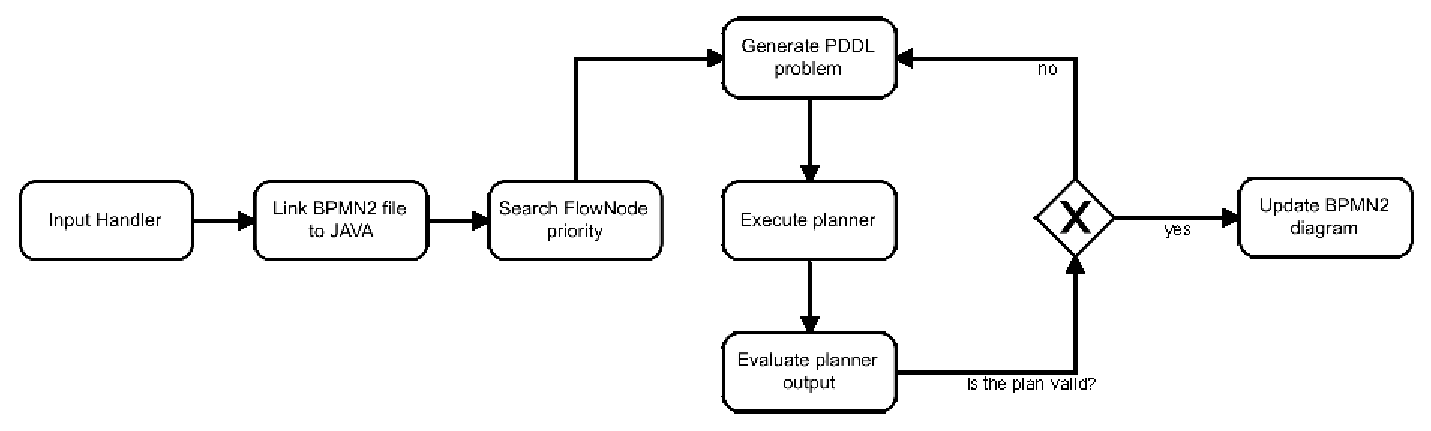
\includegraphics[width=1\textwidth]{diagram.eps}}
		\caption{The execution of BPMNPA}
\end{figure}
\end{center}

\newpage

\section{Input Parameters}
\label{sec:456}

Up to six different input arguments may be required for a correct execution of BPMNPA.
Some of them are mandatory to generate a positive outcome, while the others will allow the user to create more specific plans. The additional arguments allow the user to specify certain parameters, these can be used to modify the plan metrics. 

\paragraph{Mandatory input parameters}
\begin{itemize}

   \item[String] that we will call "planner", which has the aim of specifying the usage of the planner and the address of the executable in the file-system. The string needs to contain the keywords: \texttt{domain}, \texttt{prob} and \texttt{output}. Such keywords will be substituted with the proper sub-strings at run-time. 
   Such solution has been outlined in order to facilitate a future  improvement with the aim to establish a compatibility of BPMNPA with other planners than LPG-td. 
   It is not an easily understandable way to specify the parameter, but it has plenty of versatility and allows the user to specify optional setting for the planner execution. 
   
 	\item[String] that we will call "domain", which has the aim of specifying the path in the file-system of the PDDL domain file. This file needs to contain all the necessary elements to grant the correct execution of LPG-td such as: the name of the domain, the requirements, predicates and actions. If the user intend to use the other available parameters to specify some PDDL metrics, then it is mandatory for the domain file to contain the Functions PDDL Object.
	
	\item[String] that we will call "bpmn", which has the aim of specifying the path in the file-system of the BPMN2 compliance file. 


	\item[String] that we will call "from", which has the aim of specifying the ID of the BPMN Flow Object that will be used to set the initial states and objects in the PDDL problem. This parameter has been designed to allow the user to specify the element where the BPMN simulation (or execution) stops due to an error and cannot restore itself to reach a satisfying state or, more easily, the element from which the user decide to create a new plan. 


	\item[String] that we will call "pddl", which represents the path in the file-system of a directory containing the PDDL representations of the Flow Objects of the Business Process Diagram. 
	Every Flow Object of the BPD should have a PDDL file associated, such file must have as name the ID of the element and no file extension. 
	Furthermore, it is required that the file referring to the BPMN element used in the parameter "from" contains at least the "objects" and the "init" PDDL Objects while the files that represents the other elements must contain at least the "goal" PDDL Object.
	
\end{itemize}

\newpage
\paragraph{Optional input parameters}
\begin{itemize}
	\item[Integer] that we will call "distance", which has the aim of specifying the max number of actions that a plan can contain to be valid. It has been designed to permit the user to specify which aspect has to be prioritize, less actions added to the BPD or a BPD with lesser deviation from the original appearance.
	 
	\item[String] that we will call "max", which has the aim of specifying which metric should be maximized while searching a new plan, to use this argument it is necessary a compliance with the PDDL domain file about metrics and functions.
	
	\item[String] that we will call "min", which has the aim of specifying which metric should be minimized while searching a new plan, to use this argument it is necessary a compliance with the PDDL domain file about metrics and functions.\footnote{Only one between "max" and "min" parameters can be specified at the time.}

\end{itemize}

\begin{lstlisting}[caption=Input example with only mandatory parameters using bash.]
./BPMNPA --planner "./lpg-td -o domain -f prob -out output -n 1" --domain "domain.pddl" --bpmn "file.bpmn2" --from "Task_1" --pddl "./bpmnelements/"
\end{lstlisting}

\begin{lstlisting}[caption=Input example with optional parameters using bash.]
./BPMNPA --planner "./planner/lpg-td -o domain -f prob -out output -n 1" --domain "pddl/domain0.pddl" --bpmn "bpmn/file.bpmn2" --from "StartEvent_1" --pddl "bpmnelements/" --deviation "6" --min "(+ (price) (fuel-usage))"
\end{lstlisting}
	


\section{Transforming Plans into Business Processes}
\label{sec:456}
BPMNPA will return to the user a modified Business Process Diagram, with a new plan drawn in it. 
The new plan is generated by the planner and needs to be parsed and transformed from text to BPMN elements. 
To accomplish this, it is necessary to analyze firstly the structure of the Business Process Diagram and secondly the structure of the PDDL plan. In total, we have identified three principles that we will follow in the transposition from PDDL to BPMN.

\begin{itemize}  
\item The plan generated goes from a Flow Object to another Flow Object and in the initial path between those elements a diverging Exclusive Gateway was present without the relative converging Exclusive Gateway. In this case other plans must be generated setting as goal an element for every other branch of the outgoings Sequence Flow of the diverging Exclusive Gateway.

\item The plan generated contains actions with the same temporal slot, then the representation of those actions will be confined between a diverging Parallel Gateway and a converging Parallel Gateway.

\item Any single action will be represented as a Task element, with a random alphanumeric string as ID and with the action name as Task name.
\end{itemize}


With respect to the three previous guidelines, BPMNPA will create Task element, Parallel Gateway element and Sequence Flow element. Each Flow Object (Task and Gateway) will be linked through a Sequence Flow with another BPMN2 element, no isolated object will be created.

\newpage

\begin{lstlisting}[caption=Planner output example. In this case the first and the second actions can be executed in any order.]
0:   (ACTION0 A) [1]
0:   (ACTION0 B) [1]
1:   (ACTION1 C) [1]
2:   (ACTION2 A B) [1]
2:   (ACTION2 B C) [1]
2:   (ACTION2 C A) [1]
3:   (ACTION3 A B C) [1]
\end{lstlisting}


\begin{figure}[h!]
	\centering
	\begin{subfigure}[b]{0.7\linewidth}
    	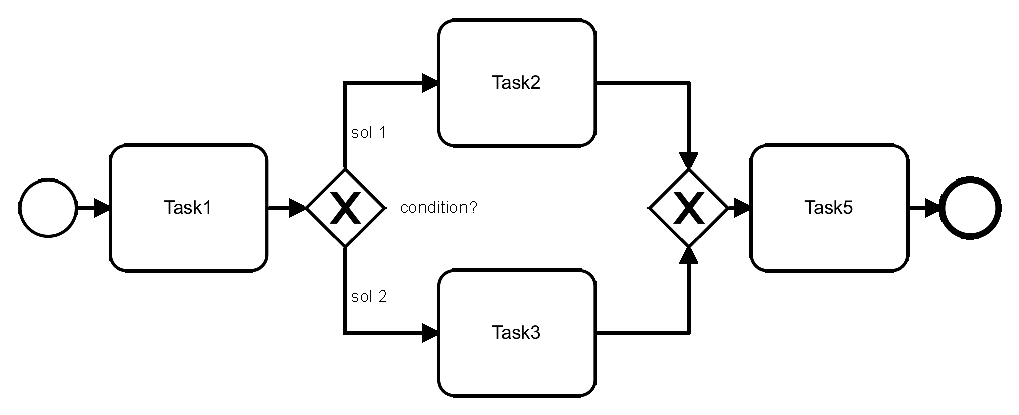
\includegraphics[width=\linewidth]{examplepre.eps}
    	\caption{The initial Business Process Diagram.}
  	\end{subfigure}
	\begin{subfigure}[b]{1\linewidth}
    	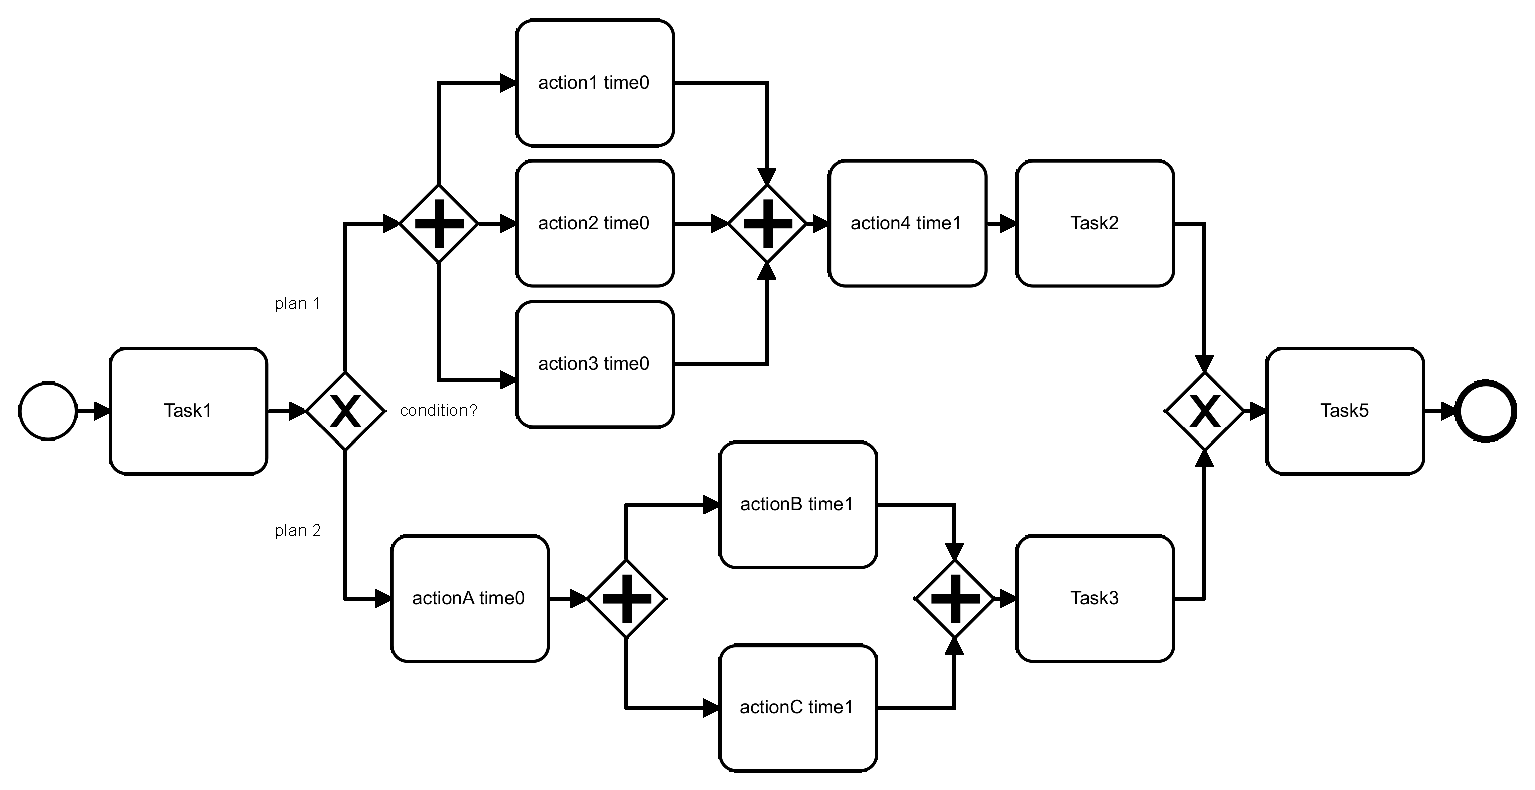
\includegraphics[width=\linewidth]{examplep.eps}
    	\caption{The Business Process Diagram after launching BPMNPA.}
  	\end{subfigure}
	\caption{An example of the execution results.}
	\label{fig:coffee}
\end{figure}
		\newpage	
		
\chapter{Implementation details}
\label{cha:789}
In this chapter some particular algorithms and implementation decisions of the prototype will be displayed.


\section{Load BPMN2 definitions in Java Objects}
\label{sec:456}
A fundamental step in the developing phase, to grant an easy access to the BPMN2 elements, it is accomplished by the following piece of code. Such code will grant the possibility to visit the object \texttt{Definitions def} as a tree. \texttt{Definitions def} contains all the BPMN2 elements of the file present at the URL location.

\begin{lstlisting}[caption=load BPMN in Java.][language=Java]

void init(String URL) {
	File file = new File(URL);

	// Create a resource set.
	ResourceSet resourceSet = new ResourceSetImpl();

	// Register the default resource factory
	resourceSet.getResourceFactoryRegistry().getExtensionToFactoryMap().put("bpmn2",
			new Bpmn2ResourceFactoryImpl());

	// Register the package
	Bpmn2Package ecorePackage = Bpmn2Package.eINSTANCE;

	// Get the URI of the model file.
	URI fileURI = URI.createFileURI(file.getAbsolutePath());

	// Demand load the resource for this file.
	this.setResource(resourceSet.getResource(fileURI, true));

	try {
		getResource().save(Collections.EMPTY_MAP);
	} catch (IOException e) {}

	DocumentRoot doc = null;
	for (int i = 0; i < getResource().getContents().size(); i++) {
		if (getResource().getContents().get(i) instanceof DocumentRoot) {
			doc = (DocumentRoot) getResource().getContents().get(i);
			break;
		}
	}

	Definitions def = null;
	if (doc != null) {
		def = doc.getDefinitions();
	}
}
\end{lstlisting}


\section{Breadth-First-Search on Business Process Diagram}
\label{sec:456}
The BPMN diagram is treated as a collection of direct graphs, considering Flow Objects as vertex and Sequence Flows as edges.

In order to visit the BPMN diagram the popular algorithm breadth-first-search (BFS) on direct graphs has been modified.
Using the BFS algorithm, the graph's nodes are visited in distance order from the starting node, where the distance is defined as minimum number of edge to pass through from the starting vertex. Since the BFS firstly visits the nearest vertex and then the furthest ones, this order is used to mark the nodes priority. 
Displayed below an extract of the BFS on BPMN algorithm.

\begin{lstlisting}[caption=BFS on Business Process Diagram.][language=Java]
void bpmn2_bfs(String from) {

	// declare DataStructures for the BFS execution.
	Queue<FlowNode> S = new LinkedList<FlowNode>();
	Map<String, Boolean> visitato = new HashMap<String, Boolean>();

	// find the start FlowNode and init the DataStructures.
	FlowNode start = null;
	for (RootElement re : def.getRootElements()) {
		if (re instanceof Process) {
			Process p = (Process) re;
			for (FlowElement fe : p.getFlowElements()) {
				if (fe instanceof FlowNode) {
					if (fe.getId().equals(from)) {
						start = (FlowNode)fe;
					}
				}
				visitato.put(fe.getId(), false);
			}
		}
	}
	S.add(start);
	visitato.put(start.getId(), true);

	// cycle through all the nodes following FlowNode "from".
	while(! S.isEmpty()) {
		FlowNode u = S.poll();		
		// ---------------------- //
		// --- vertex actions --- //
		// ---------------------- //

		for (SequenceFlow sf : u.getOutgoing()) {
			FlowNode dst = sf.getTargetRef();
				if (! visitato.get(dst.getId())) {
				visitato.put(dst.getId(), true);
				S.add(dst);
			}
			// -------------------- //
			// --- edge actions --- //
			// -------------------- //
		}
	}
}
\end{lstlisting}


\section{Problem generation, planner execution and output evaluation}
\label{sec:456}

To manage all the PDDL relative section we have done a massive use of file reading and file writing operations.

% pg
The generation of a PDDL problem needs to access the domain file and two problem file of the BPMN elements.
The domain file is needed in order to retrieve the \texttt{domain name}.
The \texttt{domain name} needs to be the same in the domain file and in the problem file.

One of the PDDL problem files belong to the BPMN element from which the new plan needs to start, from such file we will extract the Objects PDDL Object and the Init PDDL Object. These two objects describe the initial resources available to develop a plan.

The other PDDL problem file belongs to the BPMN element in which we plan to stop. From this file we will extract the Goal PDDL Object, which will represent the desired end states of the plan.

All the data gathered are going to be parsed, checked for the correct syntax and written in a newly created problem PDDL file. Furthermore, if "min" or "max" input parameters has been used, the Metrics PDDL Object, with the proper configuration, is added to the newly generated PDDL problem file.

%planner
The input parameter inserted by the user about the planner will probably look like this "\texttt{./LPG-td -o domain -f prob -out output -n 1}". BPMNPA handles the substitutions of the following pieces: the substring \texttt{domain} with the URL of the PDDL domain, the substring \texttt{prob} with the URL of the PDDL problem just generated, the substring \texttt{output} with the same URL of \texttt{prob} replacing the sub-string "\texttt{.pddl}" with "\texttt{-output}".
Furthermore, BPMNPA will start the execution of the planner with the parameters previously described.

%ov
Once the planner has completed successfully the generation of the new plan, the output file are analyzed. 
If there is no output file, it means that the planner returned \texttt{no solution} as result, otherwise the number of actions contained in the plan will be counted. 
If the number of actions exceed the value of the parameter \texttt{distance} specified by the user, then the plan is not valid and a new plan must be generated using another Flow Object. In the other case the plan will be considered valid and the actions will be parsed.


\section{BPMN Update}
\label{sec:456}
Given a plan parsed from a planner output, it is possible to modify a BPMN2 file adding the actions discovered. The action set will be represented as Task element, which will have as name the name of the action and as ID a random alphanumeric string. If a set of actions are supposed to be executed in the same temporal slot, a diverging Parallel Gateway will link the set of actions with the same temporal slot to the previous action, while a converging Parallel Gateway will link the set of actions with the next one.

New BPMN2 elements will be generated with the \texttt{Bpmn2Factory} class which will create and initiate the BPMN element. To link Flow Objects between each other some Sequence Flow are created and with their method \texttt{setSourceRef(FlowNode)} and \texttt{setTargetRef(FlowNode)} the link is established.
To add to the diagram the new objects created it is necessary to use a BPMN2 Process object, from the Process get the FlowElement list and add the new elements to such list. Same procedure must be adopted with the BPMN2 Lane object. The main difference using Lanes consist into adding only the new FlowNodes and not the SequenceFlows.

\begin{lstlisting}[caption=Example of the creation of new Tasks and SequenceFlows.]

	Task from = Bpmn2Factory.eINSTANCE.createTask();
	from.setName("from");

	Task to = Bpmn2Factory.eINSTANCE.createTask();
	to.setName("to");

	SequenceFlow sf = Bpmn2Factory.eINSTANCE.createSequenceFlow();
	sf.setSourceRef(from);
	sf.setTargetRef(to);

	// add to the process
	process.getFlowElements().add(from);
	process.getFlowElements().add(to);
	process.getFlowElements().add(sf);

	// add to the lane
	lane.getFlowNodeRefs().add(from);
	lane.getFlowNodeRefs().add(to);

\end{lstlisting}

At this point the BPMN2 file will contain the added Flow Elements, but a last step is mandatory to have a correct graphical representation in a BPMN2 diagram. 
Some BPMN Viewers are able to recreate the \texttt{BPMNDiagram} XML tag using the processes and collaborations described in the \texttt{Definitions} XML tag, for this reason an easy and fast way to allow the correct representation is to delete from \texttt{Definitions def} all \texttt{BPMNdiagram} tags and their content.

If a BPMN Viewer not supporting this feature is utilized, a \texttt{BPMNShape} or a \texttt{BPMNEdge} must be created using the \texttt{BpmnDiFactory} class for every change in the \texttt{Definitions def}. The new elements created need to be added to the correct \texttt{BPMNDiagram} tag contained in the BPMN \texttt{Definitions def}.

\begin{lstlisting}[caption=Remove all BPMNDiagram tags from the BPMNDefinitions.]
	def.getDiagrams().removeAll(def.getDiagrams());
\end{lstlisting}

		\newpage
		
\chapter{Evaluation}
\label{cha:789}

The evaluation of the prototype BPMNPA with real-life BPMN diagrams aims to verify the effectiveness of the prototype in generating meaningful BPMN diagram given the correct input parameters.
Specifically, three popular BPMN diagrams has been taken in exam\cite{bpmn2examples}, for every BPMN file a PDDL domain and some PDDL problems have been generated.
In the next sections we will illustrate and discuss how the real-world cases has been modified by the execution of BPMNPA.

\section{Pizza Delivery}
\label{sec:456}
On a modified version of "The Pizza Collaboration" Business Process Diagram we execute BPMNPA. The aim of this test case is to find an alternative path to the standard execution of the BPMN diagram using the set of actions defined in the domain. The diagram generated by BPMNPA represent a viable path to reach the Task "Receive payment" using a newly created set of Tasks and Parallel Gateways.
\begin{center}
\begin{figure}[h!]
		\centerline{\includegraphics[width=1\textwidth]{pizza.eps}}
		\caption{A modified version of the Pizza Collaboration after an alternative path search.}
\end{figure}
\end{center}


\section{Shipment Process}
\label{sec:456}
The next BPMN diagram describes the shipment process of hardware. A process engineer may want to explore the possible ways to optimize this process making its execution faster or cheaper.

With the prototype we obtain a new BPMN diagram inserting a new path for the warehouse worker Lane. This new path aim to reduce the time taken to execute the actions. It has been considered a scenario where in the same warehouse there are multiple packages with the same characteristic, to make the package gathering less expensive. The worker now decides to pick the package within the minor distance between the package location and the pick-area instead of the nearest package to the warehouse worker, diminishing the walk time.
\begin{center}
\begin{figure}[h!]
		\centerline{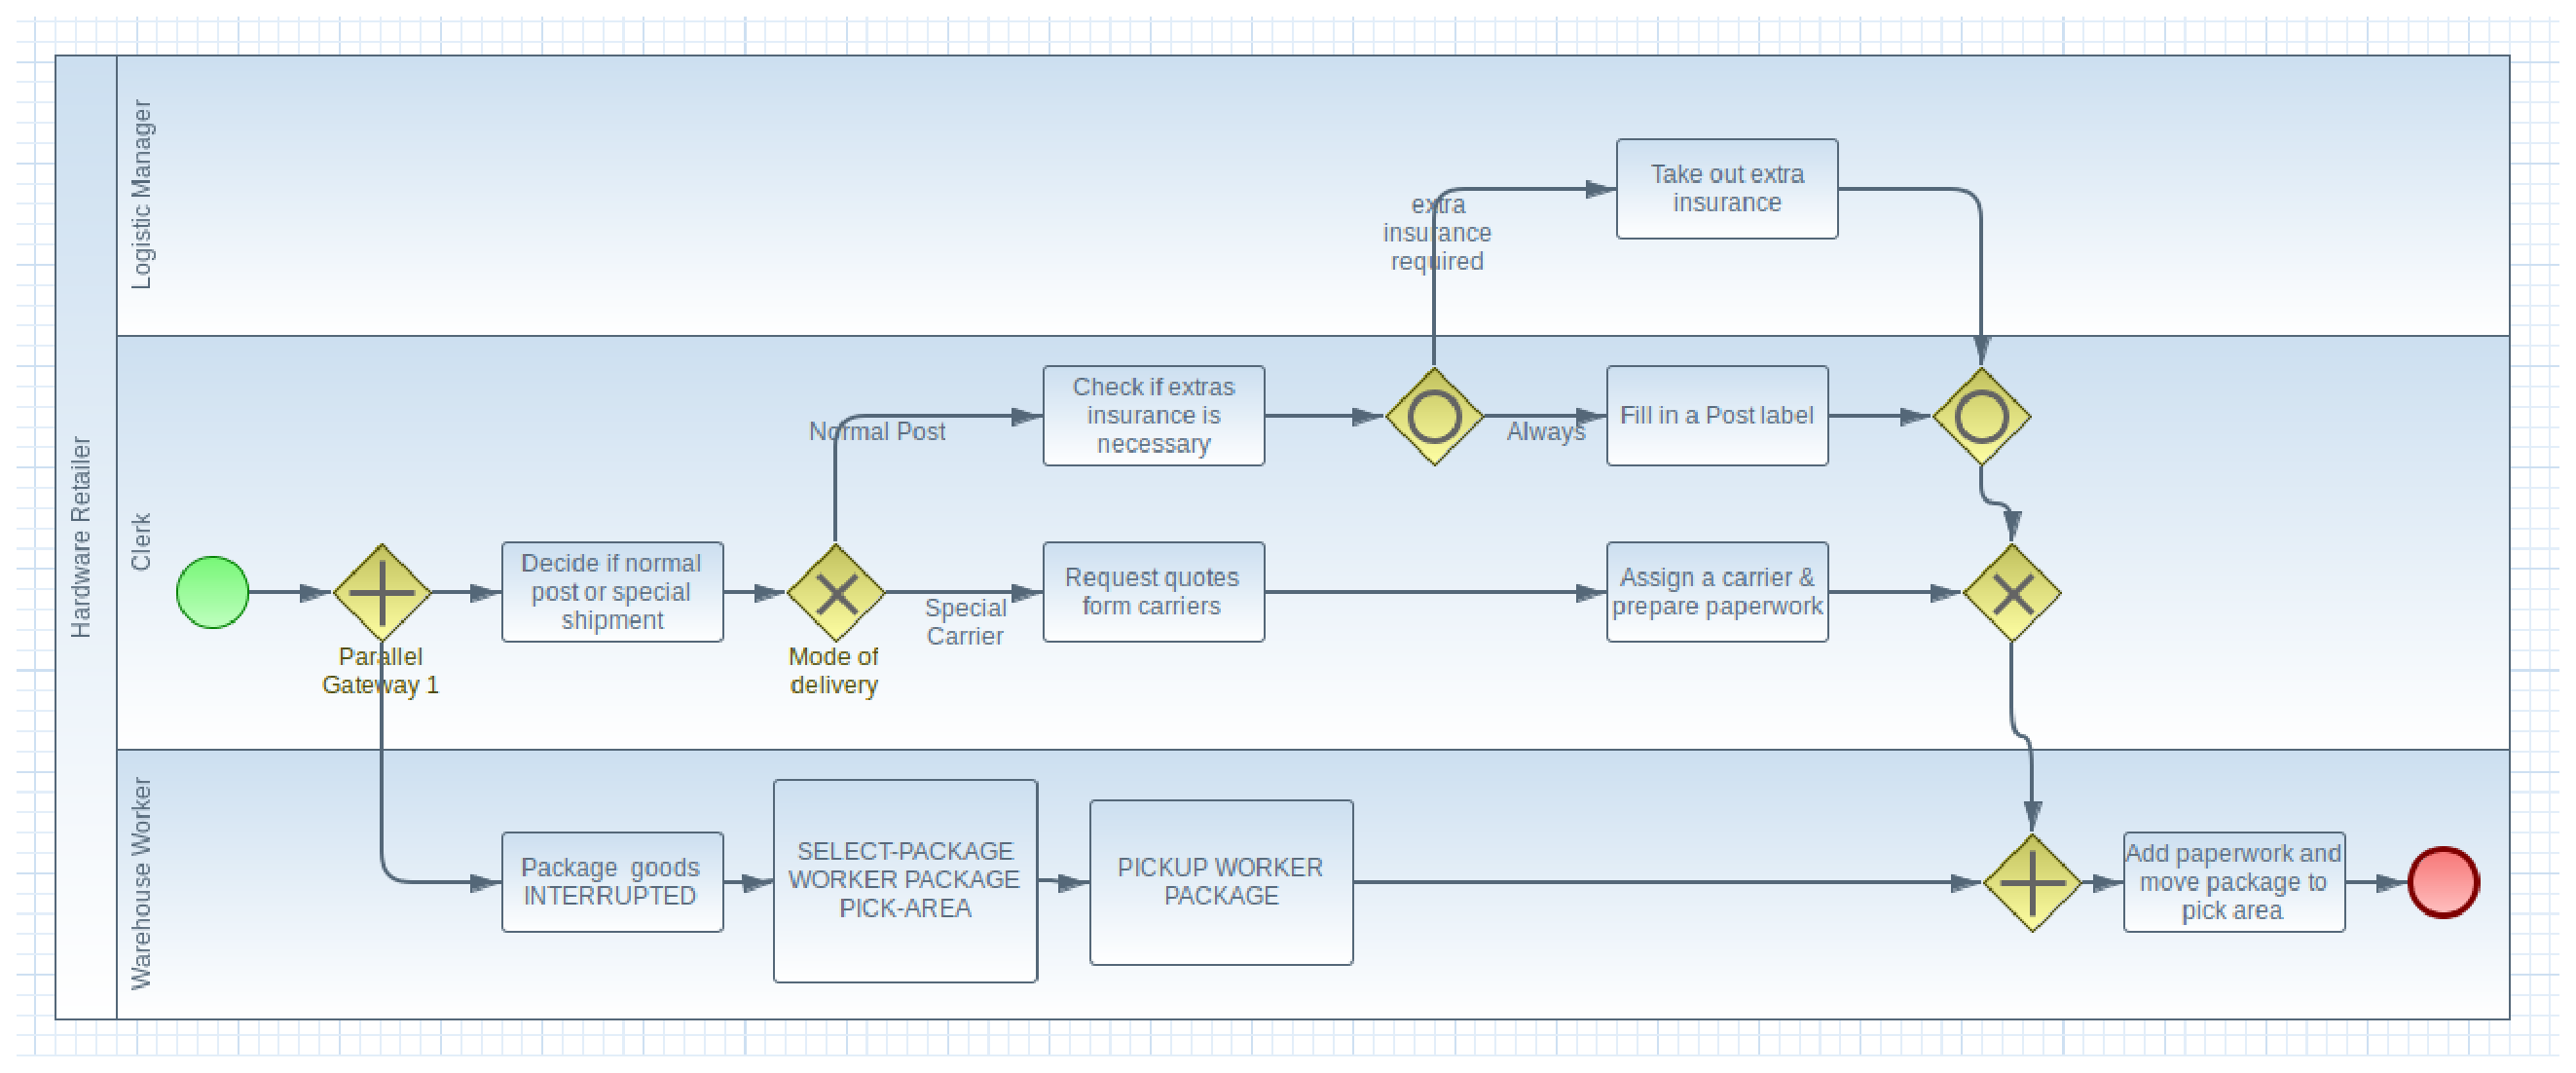
\includegraphics[width=0.8\textwidth]{warehouse.eps}}
		\caption{The Shipment Process optimized to reduce walk-time.}
\end{figure}
\end{center}

\section{Nobel Prize Example}
\label{sec:456}
In this case we considered a run-time error during the execution of the task "Discuss Nominations (meeting 1)" in the Noble Assembly Lane. We have considered the task to have as precondition the successful completion of "Submit Report with Recommendations" and as post-conditions the end of the meeting.


We consider that the run-time error, in this case, has been thrown by the fact that the meeting can start only if at-least four people are present. BPMNPA has created a new set of elements in order to exit this error state and restore the execution, by using available agents, to fulfill the goals of the Task "Discussion Nominations (meeting 1)" and to make feasible the execution of "Discussion Nominations (meeting 2)".

\begin{center}
\begin{figure}[h!]
		\centerline{\includegraphics[width=1\textwidth]{noble.eps}}
		\caption{The result of recovering a run-time error in the Nobel Prize example.}
\end{figure}
\end{center}

		
		% conclusioni
		\newpage		
		\chapter*{Conclusions} % senza numerazione
\label{Conclusions}

\addcontentsline{toc}{chapter}{Conclusions} % da aggiungere comunque all'indice


%obbiettivi della tesi 
The main goal of the thesis was to present the BPMNPA application prototype and to explore the possible interactions between PDDL and BPMN. Once that we have found a way to link this two technologies using planners and plug-ins, we aimed to find out how to act on BPMN processes through the results of PDDL planning. 

\paragraph{Results}
Orchestration process\footnote{Orchestration process is a standard process we most commonly come across in BPMN. It typically models a single coordinating point of view.} and simple processes with a limited number of collaboration between the agents of the business process model can be analyzed with BPMNPA, in order to explore different paths from what was originally designed in the BPMN processes, to optimize processes and to handle run-time unrecoverable error. 

Yet, when using BPMNPA with real-life processes, one of the biggest flaws of the prototype emerges: diagrams with a heavy usage of collaborations and communications between processes will result in a lack of valid outputs.
Furthermore, when using real-world examples has become clear that Lanes containing only one Flow Object cannot be taken as starting point for the BPMNPA execution.

\paragraph{Future Works}
A step further can be done to increase the functionality of this prototype. Indeed, the compatibility with many planner may be established with a deep check on the input parameters values and modifying the way how output parsing is done.

Many more BPMN elements can be supported as Message Flow and Data Objects, and 
PDDL files may be automatically created and initialized with the basic requirements for a planner execution for every new BPMN element added to the diagram. 
Furthermore, PDDL definitions of BPMN elements nowadays can be specified by the BPMN engineer, directly in the BPMN modeler, during the construction of the diagram. Indeed, adding support to this technology may improve by far the organization and usability of this prototype.



		
	\endgroup

\newpage
% --------------- bibliografia --------------- %
	% aggiunta del capitolo nell'indice
	\addcontentsline{toc}{chapter}{Bibliography}
	
	% stile con ordinamento alfabetico in funzione degli autori
	\bibliographystyle{plain}
	\bibliography{./assets/other/biblio}
	
	
	
% --------------- allegato --------------- %	
%	\titleformat{\chapter}
%		{\normalfont\Huge\bfseries}{Allegato \thechapter}{1em}{}
		
	% sezione Allegati - opzionale
%\appendix
%	\input{./assets/other/allegati}


\end{document}
